\documentclass[11pt]{article}
\usepackage[utf8]{inputenc} % Required for inputting international characters
\usepackage[T1]{fontenc} % Output font encoding for international characters
\usepackage{amsmath}
\usepackage{amsfonts}
\usepackage{pifont}
\usepackage{tikz}
\usepackage[backend=biber,
style=apa,
citestyle=authoryear]{biblatex}

\addbibresource{references.bib}

\usepackage{mathpazo} % Palatino font

\begin{document}

%----------------------------------------------------------------------------------------
%	TITLE PAGE
%----------------------------------------------------------------------------------------

\begin{titlepage} % Suppresses displaying the page number on the title page and the subsequent page counts as page 1
	\newcommand{\HRule}{\rule{\linewidth}{0.5mm}} % Defines a new command for horizontal lines, change thickness here

	\center % Centre everything on the page

	%------------------------------------------------
	%	Headings
	%------------------------------------------------

	\textsc{\LARGE American Public University}\\[1.5cm] % Main heading such as the name of your university/college

	%------------------------------------------------
	%	Title
	%------------------------------------------------

	\HRule\\[0.4cm]

	{\huge\bfseries Writing Assignment MATH412}\\[0.4cm] % Title of your document

	\HRule\\[1.5cm]

	%------------------------------------------------
	%	Author(s)
	%------------------------------------------------

	\begin{minipage}{0.4\textwidth}
		\begin{flushleft}
			\large
			\textit{Author}\\
			Daniel \textsc{Justice} % Your name
		\end{flushleft}
	\end{minipage}
	~
	\begin{minipage}{0.4\textwidth}
		\begin{flushright}
			\large
			\textit{Professor}\\
			Dr. Richard \textsc{Han} % Supervisor's name
		\end{flushright}
	\end{minipage}

	%------------------------------------------------
	%	Date
	%------------------------------------------------

	\vfill\vfill\vfill
	{\large\today} % Date, change the \today to a set date if you want to be precise
	\vfill

\end{titlepage}

%----------------------------------------------------------------------------------------

\section*{2.44}

Let $G$ be a simple graph on $2k$ vertices containing no triangles.
Prove, by induction on $k$, that $G$ has at most $k^2$ edges, and give an example of a graph for which this upper bound is achieved.
(This result is often called Turán’s extremal theorem.)

\paragraph{Definitions}

The order of a graph is the number of vertices, and the size is the number of edges (\cite{chart}).
A triangle is a 3-cycle of 3 vertices and 3 edges.

\paragraph{Proposition}

If $G$ has no triangles, it has at most $k^2$ edges.

\paragraph{Base case}

$k=1, 2k=2$: By the definition of a simple graph (\cite{wilson}), $G_2$ may not contain any self-loops or multiple edges between vertices.
In the case of $k=1$ and a graph of $2k$ vertices, only one edge is possible and no triangles are possible.

\paragraph{Inductive Hypothesis}

Let $k \in \mathbb{N}$ and $G_n$ be a graph of size $n=2k$ with no triangles. Assume that

$$size(G_1) \le 1^2, size(G_2) \le 2^2, size(G_3) \le 3^2, \cdots size(G_{n}) \le (n)^2$$

\paragraph{Induction step}

We need to show that

$$size(G_{n+1}) \le (n+1)^2 \le {n \choose 2} - {\frac{n}{2} - 1 \choose 2}$$

Take the 3 vertices of a triangle and put them in two different sets.
One set has size 1 and the other size 2.
The size 2 set has an edge between the vertices in this set.
Deleting this edge removes the triangle.

Start with a complete graph where every vertex is connected to every other vertex.
Since $2k$ is even, divide the collection of vertices into two sets (a bipartite collection of vertices).
There are ${n \choose 2}$ edges in a complete graph of size $n$.
In each of the bipartite sets, there are $\frac{n}{2}$ vertices.
Each vertex is connected to every other vertex in this set, so there are ${\frac{n}{2} - 1 \choose 2}$ edges in this subset.
This leaves $\frac{n}{2}^2=k^2$ edges between the sets, and adding any other edge would create a triangle.
Thus the number of edges in the bipartite graph are the maximum number of edges for a graph of $size(n)$ that has no triangles.

$$n = 2k$$

$$
\begin{aligned}
	size(G_{n+1}) \le (k + 1)^2 \le {n + 1 \choose 2} - 2{(\frac{n}{2} + 1) - 1 \choose 2} \\
	\le {2k + 1 \choose 2} - 2{(k + 1) - 1 \choose 2} \\
	\le \frac{(2(k + 1))!}{2(2k + 1 - 2)!} - 2{k \choose 2} \\
	\le \frac{2(k+1)(2(k+1) - 1)}{2} - \frac{2(k+1)(k+1-1)}{2} \\
	\le (k+1)(2(k+1) - 1) - (k+1)(k) \\
	\le (k+1)(2k+1) - k^2 +k \\
	\le 2k^2+3k+1 - k^2 +k \\
	\le k^2 + 2k + 1 \\
	\le (k+1)^2 \\
\end{aligned}
$$

as desired.

\paragraph{Conclusion}

The number of edges in the bipartite graph are the maximum number of edges for a graph of $size(2k)$ that has no triangles.

$\square$

\paragraph{Example}

Given $k=3$, here is a graph of order $2k$ and size $k^2$.
Adding any other edge would result in a triangle.
This is clearer if we rearrange the graph into its bipartite sets.
The following graphs are isomorphic.

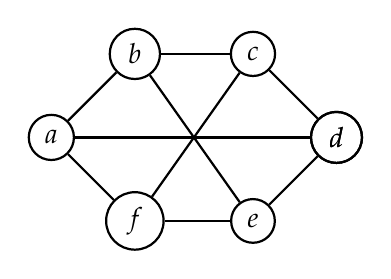
\begin{tikzpicture}[node distance={15mm}, thick, main/.style = {draw, circle}]
\node[main] (a) {$a$};
\node[main] (b) [above right of=a] {$b$};
\node[main] (c) [right of=b] {$c$};
\node[main] (d) [below right of=c] {$d$};
\node[main] (d) [below right of=c] {$d$};
\node[main] (f) [below right of=a] {$f$};
\node[main] (e) [right of=f] {$e$};
\draw[-] (a) -- (b);
\draw[-] (b) -- (c);
\draw[-] (c) -- (d);
\draw[-] (d) -- (e);
\draw[-] (e) -- (f);
\draw[-] (f) -- (a);
\draw[-] (a) -- (d);
\draw[-] (b) -- (e);
\draw[-] (f) -- (c);
\end{tikzpicture}
\quad
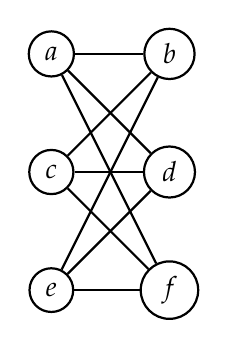
\begin{tikzpicture}[node distance={15mm}, thick, main/.style = {draw, circle}]
\node[main] (a) {$a$};
\node[main] (c) [below of=a] {$c$};
\node[main] (e) [below of=c] {$e$};
\node[main] (b) [right of=a] {$b$};
\node[main] (d) [right of=c] {$d$};
\node[main] (f) [right of=e] {$f$};
\draw[-] (a) -- (b);
\draw[-] (b) -- (c);
\draw[-] (c) -- (d);
\draw[-] (d) -- (e);
\draw[-] (e) -- (f);
\draw[-] (f) -- (a);
\draw[-] (a) -- (d);
\draw[-] (b) -- (e);
\draw[-] (f) -- (c);
\end{tikzpicture}

\section*{2.45}

\subsection*{(i)}
Prove that, if two distinct cycles of a graph $G$ each contain an edge $e$, then $G$ has a cycle that does not contain $e$.

\subsection*{Proof}

The smallest cycle possible is a triangle where every vertex has degree 2.
Combining two triangles on any edge results in a graph of order 4 and size 5 (6 edges - 1 shared edge).
This graph must contain two edges of degree 3.
Deleting the shared edge results in a graph of order 4 and size 4 where every vertex has a degree of 2.
This new graph must contain a cycle because there are no vertices of degree 1.

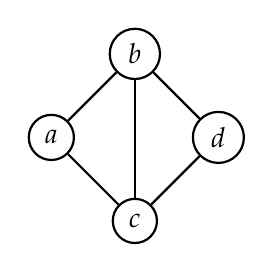
\begin{tikzpicture}[node distance={15mm}, thick, main/.style = {draw, circle}]
\node[main] (a) {$a$};
\node[main] (b) [above right of=a] {$b$};
\node[main] (c) [below right of=a] {$c$};
\node[main] (d) [below right of=b] {$d$};
\draw[-] (a) -- (b);
\draw[-] (a) -- (c);
\draw[-] (b) -- (d);
\draw[-] (c) -- (d);
\draw[-] (b) -- (c);
\end{tikzpicture}
\quad
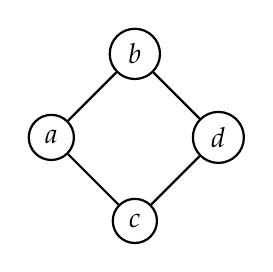
\begin{tikzpicture}[node distance={15mm}, thick, main/.style = {draw, circle}]
\node[main] (a) {$a$};
\node[main] (b) [above right of=a] {$b$};
\node[main] (c) [below right of=a] {$c$};
\node[main] (d) [below right of=b] {$d$};
\draw[-] (a) -- (b);
\draw[-] (a) -- (c);
\draw[-] (b) -- (d);
\draw[-] (c) -- (d);
\end{tikzpicture}

$\square$

\subsection*{(ii)}
Prove a similar result with 'cycles' replaced by 'cutsets'.

Prove that, if two distinct cutsets of a graph $G$ each contain an edge $e$, then $G$ has a cutset that does not contain $e$.

\subsection*{Proof}

Two distinct cutsets containing a common edge $e$ have at least two vertices in common.
At a minimum:
$$C_1 = \{\{a, b\}, \{b, c\}\}, C_2 = \{\{a, b\}, \{a, c\}\}$$

The two cutsets must have some other vertex not in common or they would not be distinct sets.

\begin{tikzpicture}[node distance={15mm}, thick, main/.style = {draw, circle}]
\node[main] (b) {$b$};
\node[main] (a) [above right of=1] {$a$};
\node[main] (c) [below right of=a] {$c$};
\draw[-] (a) -- (b);
\draw[-] (a) -- (c);
\draw[-] (b) -- (c);
\end{tikzpicture}

$\square$

\printbibliography

\end{document}
